\documentclass{article}\usepackage[]{graphicx}\usepackage[]{color}
%% maxwidth is the original width if it is less than linewidth
%% otherwise use linewidth (to make sure the graphics do not exceed the margin)
\makeatletter
\def\maxwidth{ %
  \ifdim\Gin@nat@width>\linewidth
    \linewidth
  \else
    \Gin@nat@width
  \fi
}
\makeatother

\definecolor{fgcolor}{rgb}{0.345, 0.345, 0.345}
\newcommand{\hlnum}[1]{\textcolor[rgb]{0.686,0.059,0.569}{#1}}%
\newcommand{\hlstr}[1]{\textcolor[rgb]{0.192,0.494,0.8}{#1}}%
\newcommand{\hlcom}[1]{\textcolor[rgb]{0.678,0.584,0.686}{\textit{#1}}}%
\newcommand{\hlopt}[1]{\textcolor[rgb]{0,0,0}{#1}}%
\newcommand{\hlstd}[1]{\textcolor[rgb]{0.345,0.345,0.345}{#1}}%
\newcommand{\hlkwa}[1]{\textcolor[rgb]{0.161,0.373,0.58}{\textbf{#1}}}%
\newcommand{\hlkwb}[1]{\textcolor[rgb]{0.69,0.353,0.396}{#1}}%
\newcommand{\hlkwc}[1]{\textcolor[rgb]{0.333,0.667,0.333}{#1}}%
\newcommand{\hlkwd}[1]{\textcolor[rgb]{0.737,0.353,0.396}{\textbf{#1}}}%
\let\hlipl\hlkwb

\usepackage{framed}
\makeatletter
\newenvironment{kframe}{%
 \def\at@end@of@kframe{}%
 \ifinner\ifhmode%
  \def\at@end@of@kframe{\end{minipage}}%
  \begin{minipage}{\columnwidth}%
 \fi\fi%
 \def\FrameCommand##1{\hskip\@totalleftmargin \hskip-\fboxsep
 \colorbox{shadecolor}{##1}\hskip-\fboxsep
     % There is no \\@totalrightmargin, so:
     \hskip-\linewidth \hskip-\@totalleftmargin \hskip\columnwidth}%
 \MakeFramed {\advance\hsize-\width
   \@totalleftmargin\z@ \linewidth\hsize
   \@setminipage}}%
 {\par\unskip\endMakeFramed%
 \at@end@of@kframe}
\makeatother

\definecolor{shadecolor}{rgb}{.97, .97, .97}
\definecolor{messagecolor}{rgb}{0, 0, 0}
\definecolor{warningcolor}{rgb}{1, 0, 1}
\definecolor{errorcolor}{rgb}{1, 0, 0}
\newenvironment{knitrout}{}{} % an empty environment to be redefined in TeX

\usepackage{alltt}

%
% Paquets basics: posar-los sempre
%
\usepackage[utf8]{inputenc}
\usepackage[T1]{fontenc}
%\usepackage[spanish, catalan]{babel}
\usepackage[english,spanish]{babel}
\usepackage{url}
%\usepackage[pdftex]{graphicx}
\usepackage{underscore}


% 
% Paquets opcionals: posar-los quan sapiguem si cale i que coi fan ...
%
\usepackage{times}
\usepackage{amsmath}
\usepackage{amssymb,amsfonts,textcomp}
\usepackage{array}
\usepackage{hhline}


% \textwidth=6.2in
% \textheight=8.5in
% %\parskip=.3cm
% \oddsidemargin=.1in
% \evensidemargin=.1in
% \headheight=-.3in



\newcommand{\R}{\textbf{R}\,}
\newcommand{\RFI}{\textbf{R}}

\newcommand{\Rfun}[1]{{\texttt{#1}}}
\newcommand{\Robj}[1]{{\texttt{#1}}}
\newcommand{\Rpac}[1]{{\textit{#1}}}   
\newcommand{\Rfunction}[1]{{\texttt{#1}}}
\newcommand{\Robject}[1]{{\texttt{#1}}}
\newcommand{\Rpackage}[1]{{\textit{#1}}}
\newcommand{\Rclass}[1]{{\textit{#1}}}
\newcommand{\bit}{\begin{itemize}}
\newcommand{\eit}{\end{itemize}}
\newcommand{\ben}{\begin{enumerate}}
\newcommand{\een}{\end{enumerate}}

\newcommand{\classdef}[1]{%
  {\em #1}
}


\title{Building and validating predictors using \R \\ and the CMA package}

\author{Alex Sánchez\\
Estad\'istica i Bioinform\`atica\\
Department d'Estadística. Universitat de Barcelona}

\bibliographystyle{plain}

% \includeonly{file1, file2, ...} % Por si se quiere romper el documento en subdocumentos elaborables separadamente
\IfFileExists{upquote.sty}{\usepackage{upquote}}{}
\begin{document}

\maketitle

\tableofcontents






\section{Introduction}

A common task in bioinformatics is to build and validate predictor -often called a classifier- to distinguish between two or more biological classes based on a series of biological features such as genes, microRNA, metabolites (or, more recently, a combination of some of these).

Our goal here is to illustrate the \emph{standard process} such as
described by Sanchez et alt. (\cite{Sanchez2012}) or by  \cite{Dziuda2010} and summarized
 in the follwing two figures.

Figure \ref{workflow} illustrates the basics blocks on which the biomarker discovery process can be arbitrarily divided. Figure \ref{validation} illustrates how to use cross-validation to build and validate a biomarker in such a way that unbiased estimates of generalization error can be obtained.

\begin{figure}
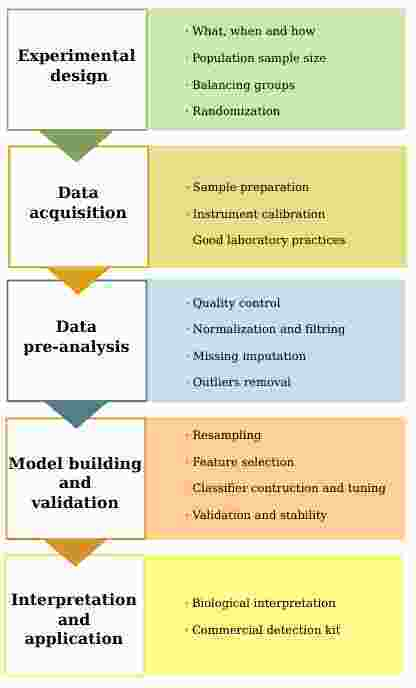
\includegraphics[width=0.7\textwidth]{images/biomarkerDiscoveryWorkflow}
\caption{Basics steps in biomarker discovery\label{workflow}}
\end{figure}


\begin{figure}
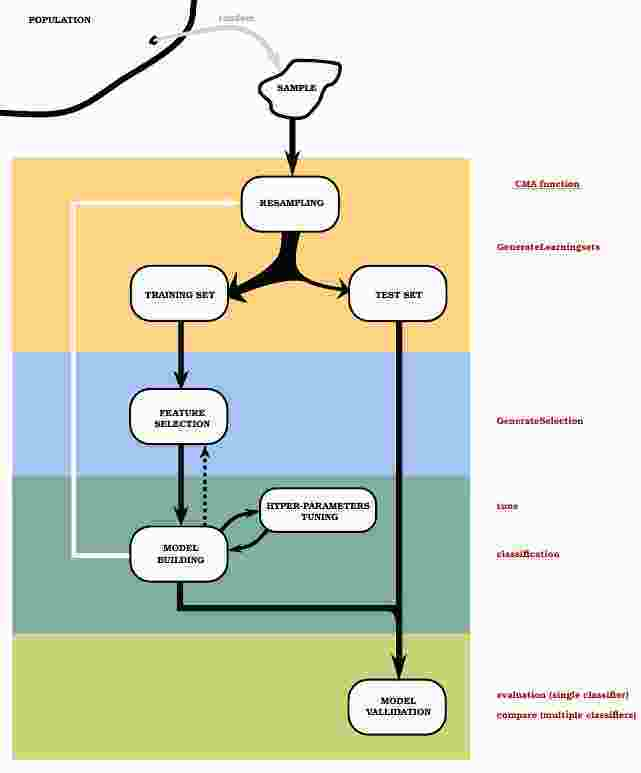
\includegraphics[width=0.7\textwidth]{images/biomarkerValidationScheme}
\caption{Basic steps of cross-validation\label{validation}}
\end{figure}

\subsection{The CMA package}

There are many packages in \R to apply each of the many available
classification methods.  Some of them such as \texttt{caret}, \texttt{CMA} or \texttt{MLtools} also support the process of
building and validating a classifier based on testing a set of
different approaches on a set of samples using an appropriate
cross-validation approach. 

Here we rely on the Bioconductor \texttt{CMA} (``Classification for MicroArrays'') package which has been
specifically designed with microarray data in mind, but can also be used with any high throughput data.

\begin{knitrout}
\definecolor{shadecolor}{rgb}{0.969, 0.969, 0.969}\color{fgcolor}\begin{kframe}


{\ttfamily\noindent\itshape\color{messagecolor}{\#\# Loading required package: e1071}}

{\ttfamily\noindent\itshape\color{messagecolor}{\#\# Loading required package: glmnet}}

{\ttfamily\noindent\itshape\color{messagecolor}{\#\# Loading required package: Matrix}}

{\ttfamily\noindent\itshape\color{messagecolor}{\#\# Loading required package: foreach}}

{\ttfamily\noindent\itshape\color{messagecolor}{\#\# Loaded glmnet 2.0-16}}

{\ttfamily\noindent\itshape\color{messagecolor}{\#\# Loading required package: randomForest}}

{\ttfamily\noindent\itshape\color{messagecolor}{\#\# randomForest 4.6-14}}

{\ttfamily\noindent\itshape\color{messagecolor}{\#\# Type rfNews() to see new features/changes/bug fixes.}}

{\ttfamily\noindent\itshape\color{messagecolor}{\#\# Loading required package: CMA}}

{\ttfamily\noindent\itshape\color{messagecolor}{\#\# Loading required package: Biobase}}

{\ttfamily\noindent\itshape\color{messagecolor}{\#\# Loading required package: BiocGenerics}}

{\ttfamily\noindent\itshape\color{messagecolor}{\#\# Loading required package: parallel}}

{\ttfamily\noindent\itshape\color{messagecolor}{\#\# \\\#\# Attaching package: 'BiocGenerics'}}

{\ttfamily\noindent\itshape\color{messagecolor}{\#\# The following objects are masked from 'package:parallel':\\\#\# \\\#\#\ \ \ \  clusterApply, clusterApplyLB, clusterCall, clusterEvalQ,\\\#\#\ \ \ \  clusterExport, clusterMap, parApply, parCapply, parLapply,\\\#\#\ \ \ \  parLapplyLB, parRapply, parSapply, parSapplyLB}}

{\ttfamily\noindent\itshape\color{messagecolor}{\#\# The following object is masked from 'package:randomForest':\\\#\# \\\#\#\ \ \ \  combine}}

{\ttfamily\noindent\itshape\color{messagecolor}{\#\# The following objects are masked from 'package:Matrix':\\\#\# \\\#\#\ \ \ \  colMeans, colSums, rowMeans, rowSums, which}}

{\ttfamily\noindent\itshape\color{messagecolor}{\#\# The following objects are masked from 'package:stats':\\\#\# \\\#\#\ \ \ \  IQR, mad, sd, var, xtabs}}

{\ttfamily\noindent\itshape\color{messagecolor}{\#\# The following objects are masked from 'package:base':\\\#\# \\\#\#\ \ \ \  anyDuplicated, append, as.data.frame, basename, cbind, colMeans,\\\#\#\ \ \ \  colnames, colSums, dirname, do.call, duplicated, eval, evalq,\\\#\#\ \ \ \  Filter, Find, get, grep, grepl, intersect, is.unsorted, lapply,\\\#\#\ \ \ \  lengths, Map, mapply, match, mget, order, paste, pmax, pmax.int,\\\#\#\ \ \ \  pmin, pmin.int, Position, rank, rbind, Reduce, rowMeans, rownames,\\\#\#\ \ \ \  rowSums, sapply, setdiff, sort, table, tapply, union, unique,\\\#\#\ \ \ \  unsplit, which, which.max, which.min}}

{\ttfamily\noindent\itshape\color{messagecolor}{\#\# Welcome to Bioconductor\\\#\# \\\#\#\ \ \ \  Vignettes contain introductory material; view with\\\#\#\ \ \ \  'browseVignettes()'. To cite Bioconductor, see\\\#\#\ \ \ \  'citation("{}Biobase"{})', and for packages 'citation("{}pkgname"{})'.}}

{\ttfamily\noindent\itshape\color{messagecolor}{\#\# \\\#\# Attaching package: 'CMA'}}

{\ttfamily\noindent\itshape\color{messagecolor}{\#\# The following object is masked from 'package:e1071':\\\#\# \\\#\#\ \ \ \  tune}}\end{kframe}
\end{knitrout}


The aim of the \texttt{CMA} package is \emph{to provide a
user-friendly environment for the evaluation of classification methods using gene expression data}. A strong focus is on combined variable
selection, hyperparameter tuning, evaluation, visualization and
comparison of (up to now) 21 classification methods from three main
fields: Discriminant Analysis, Neural Networks and Machine Learning.

Using this package a (not-so-)simple workflow for building and validating a classifier can be used
The main steps for this workflow are: 
\begin{enumerate}
\item Start with a high-throughput dataset (e.g. en expression matrix) and a vector of labels assigning each column of the dataset to a group.
\item 
Generate a given number of evaluation datasets (using \texttt{GenerateLearningsets}(.
\item 
(Optionally): Do variable selection (using \texttt{GeneSelection}).
\item 
(Optionally): Do hyperparameter tuning (using \texttt{tune}).
\item 
Perform classification using 1.-3.
\item 
Repeat steps 3--5 based on the learning sets generated in step 2 for an appropriate (wisely chosen) subset of all available methods\footnote{compBoostCMA, dldaCMA, ElasticNetCMA, fdaCMA, flexdaCMA, gbmCMA, knnCMA, ldaCMA, LassoCMA, nnetCMA, pknnCMA, plrCMA, pls_ldaCMA, pls_lrCMA, pls_rfCMA, pnnCMA, qdaCMA, rfCMA, scdaCMA, shrinkldaCMA, svmCMA}.
\item Evaluate the results from 6 using \texttt{evaluation} and/or compare the different results using the \texttt{compare} function.
\end{enumerate}

\textbf{In practice} in order to implement the workflow a series of decisions must be taken. This means that one has to decide:
\begin{itemize}
\item Which methods to use for building learning sets.
\item Which methods to use for selecting variables with best discriminating power.
\item How many variables to use when building those classifiers that cannot decide this by themselves.
\item Which classifiers to build so that the set of classifiers tested is simultaneosuly comprehensive (represents well different philosopies) and non-redundant (excludes equivalent or very similar methods).
\end{itemize}

This can be done using a nested loop that applies each gene selection
method for each sample size each learning set and each classifier.

\subsection{The data for the examples}

Although the goal of this document is to be as general as possible it
is good to recall that not all datasets are equally suitable for
classification analysis, due mainly to the fact that problems in the data can badly affect the performance of predictors obtained.

That is, if the data to be used has problems such as \emph{batch effects}, \emph{too many variables} or \emph{outliers}, this has to be dealt with before attempting to build
and compare the predictors.

Some typical preprocessing that may have to be dealt with are:
\begin{enumerate}
\item Remove outliers, 
\item Keep only groups of samples where there were individuals of both classes analyzed,
\item Remove batch effects attributable to technical questions or to experimental design,
\item Filter the data to retain only genes with a ``minimum" variability. That is, remove ``flat" features, which cannot reasonably contribute to distinguish classes but which, instead, claerly add noise.
\end{enumerate}

CMA expects the data to consist of:
\begin{itemize}
  \item a numerical matrix\footnote{Indeed for coherence with many standard \R packages CMA assumes that variables are in columns and samples in rows, that is, it works with what would be the transposed of standard expression matrices.}, 
  \item a character/factor vector with the labels describing to which group each individual begins.
\end{itemize}

In order to keep this document as much general as possible the data used to illustrate the following sections are one of those contained in the CMA package, the \texttt{khan} dataset. It consists of expression values obtained from small blue round cell tumour which
comprises 65 samples from four tumour classes.

\begin{knitrout}
\definecolor{shadecolor}{rgb}{0.969, 0.969, 0.969}\color{fgcolor}\begin{kframe}
\begin{alltt}
\hlkwd{library}\hlstd{(CMA)}
\hlkwd{data}\hlstd{(khan)}
\hlkwd{dim}\hlstd{(khan)}
\end{alltt}
\begin{verbatim}
## [1]   63 2309
\end{verbatim}
\begin{alltt}
\hlkwd{head}\hlstd{(khan[}\hlkwd{sample}\hlstd{(}\hlnum{1}\hlopt{:}\hlkwd{nrow}\hlstd{(khan),}\hlnum{10}\hlstd{),} \hlnum{1}\hlopt{:}\hlnum{5}\hlstd{])}
\end{alltt}
\begin{verbatim}
##    khanY      X2        X3        X4       X5
## 37   RMS 1.24231  0.251148 -1.092133 -2.41575
## 23   EWS 0.83824 -1.833207 -0.547144 -0.68082
## 32   RMS 0.43243 -2.700082 -0.402121  0.13077
## 33   RMS 0.89294  0.026837 -0.062620 -2.21641
## 11   EWS 1.16393 -2.686778  0.044973 -2.08506
## 22   EWS 0.76593 -2.337177 -0.694748 -1.50869
\end{verbatim}
\begin{alltt}
\hlkwd{table}\hlstd{(khan}\hlopt{$}\hlstd{khanY)}
\end{alltt}
\begin{verbatim}
## 
##  BL EWS  NB RMS 
##   8  23  12  20
\end{verbatim}
\end{kframe}
\end{knitrout}

\paragraph{Two-class vs multi-class classifiers}
Classifiers may be built for problems with two or more than two groups. We start with a simplified example which corresponds to the most common situation, that is when there are two groups. For this we take a subset of the original data, that formed by the ``EWS'' and the ``RMS'' individuals.

\begin{knitrout}
\definecolor{shadecolor}{rgb}{0.969, 0.969, 0.969}\color{fgcolor}\begin{kframe}
\begin{alltt}
\hlstd{khan2groups} \hlkwb{<-} \hlstd{khan[khan}\hlopt{$}\hlstd{khanY} \hlopt \hlkwd{c}\hlstd{(}\hlstr{"EWS"}\hlstd{,}\hlstr{"RMS"}\hlstd{),]}
\hlstd{nabX} \hlkwb{<-} \hlkwd{as.matrix}\hlstd{(khan2groups[,}\hlopt{-}\hlnum{1}\hlstd{])}
\hlstd{nabY2} \hlkwb{<-} \hlstd{labs}\hlkwb{<-}\hlkwd{as.factor}\hlstd{(khan2groups[,}\hlnum{1}\hlstd{]);}
\hlstd{nabY} \hlkwb{<-} \hlkwd{droplevels}\hlstd{(nabY2 )}
\hlkwd{table}\hlstd{(nabY)}
\end{alltt}
\begin{verbatim}
## nabY
## EWS RMS 
##  23  20
\end{verbatim}
\end{kframe}
\end{knitrout}

\section{Building and validating the predictors}

In the following sections the process of building and validating the predictor, as described in previous section, is applied to the \texttt{khan} dataset.




\subsection{Creating the learning datasets}

Ideally in classification problems one should have a completely independent test set where the classifier could be checked once it has been built on the train data. 

Given that it is not usually possible an alternative approach is to perform \emph{cross-validation} which consists of creating a certain number of splits of the data (that is different divisions of the original dataset into a train and test subset) which can later be used to train/test the predictor and whose results can be aggregated.

There are different schemes for splitting the samples into test and train subsets. Here we use  the "five-fold" and "Monte Carlo Cross--Validation" approaches, described in in the CMA vignette. Briefly,
\begin{itemize}
  \item Five-fold Cross Validation divides the data in five parts. Four are used to train the classification model and one is used to test the model. The number of possible decompositions in 4+1 parts depends on the sample size but usually no all possible combinations will be used.
  \item Monte Carlo Cross-Validation uses a ``random splitting'' scheme that is the data are randomly divided in two parts of sample sizes 1/5th and 4/5th respectively.
\end{itemize}

\begin{knitrout}
\definecolor{shadecolor}{rgb}{0.969, 0.969, 0.969}\color{fgcolor}\begin{kframe}
\begin{alltt}
\hlcom{#### NOTA: AL FER EL CÀLCUL DEFINITIU CONVE AUGMENTAR EL NOMBRE D'ITERACIONS. (per exemple a 1000)}
\hlstd{numIter} \hlkwb{<-} \hlnum{100}
\hlstd{numFold} \hlkwb{<-} \hlnum{5}
\hlstd{learnSetNames} \hlkwb{<-} \hlkwd{c}\hlstd{(}\hlstr{"fiveFold"}\hlstd{,} \hlstr{"MCCV"}\hlstd{)}
\hlkwd{set.seed}\hlstd{(}\hlnum{1234567}\hlstd{)}
\end{alltt}
\end{kframe}
\end{knitrout}




\subsection{Selecting genes}

The first important step in the process of building a classifier is \emph{variable selection}. It is very important, however, not to confound variable selection with classification. Gene selection -or variable selection- is ``only'' intended to select appropriate variables, but tells nothing about classifiers. Classification relies on variables that distinguish well samples but it looks for a more complex information, that is the ability to classify new individuals into groups.

Following the recommendations in \cite{Boulesteix2008} it is a good idea to use several, different, variable selection methods that rely on different approaches, Here we try three  gene selection methods: \emph{T-test}, \emph{Random forest} and the \emph{Lasso}.

The code below shows how to perform gene selection on the different learning sets and how to annotate and compare them.

This provides relevant information, but it is important to recall that it does not provide us with what is the goal of this document: a good classifier.

At the end of the process, once the variables and the method for combining them have been decided the classificator has to be built with all the data.



\begin{knitrout}
\definecolor{shadecolor}{rgb}{0.969, 0.969, 0.969}\color{fgcolor}\begin{kframe}
\begin{alltt}
\hlstd{selMethodNames} \hlkwb{<-} \hlkwd{c}\hlstd{(}\hlstr{"f.test"}\hlstd{,} \hlstr{"rf"}\hlstd{)} \hlcom{# , "lasso") # VALID FOR TWO GRUPS}
\hlstd{selScheme} \hlkwb{<-} \hlstr{"pairwise"}                       \hlcom{# VALID FOR TWO GRUPS}
\hlstd{schemeName} \hlkwb{<-} \hlstr{"pairwise"}
\hlcom{# selMethodNames <- c("f.test", "rf")            # VALID FOR MORE-THAN-TWO GRUPS}
\hlcom{# schemeName <- "multiclass"                     # VALID FOR MORE-THAN-TWO GRUPS}
\hlstd{numGenes2Sel} \hlkwb{<-} \hlkwd{c}\hlstd{(}\hlnum{5}\hlstd{,} \hlnum{10}\hlstd{,} \hlnum{25}\hlstd{)}
\end{alltt}
\end{kframe}
\end{knitrout}

\begin{knitrout}
\definecolor{shadecolor}{rgb}{0.969, 0.969, 0.969}\color{fgcolor}\begin{kframe}
\begin{alltt}
\hlcom{# Això no cal fer-ho perque es fa al loop principal}
\hlstd{geneSels}\hlkwb{<-} \hlkwd{list}\hlstd{()}
\hlkwa{for} \hlstd{(i} \hlkwa{in} \hlnum{1}\hlopt{:}\hlkwd{length}\hlstd{(learningSets))\{}
  \hlkwa{for} \hlstd{(j} \hlkwa{in} \hlnum{1}\hlopt{:}\hlkwd{length}\hlstd{(selMethodNames))\{}
    \hlstd{selected}  \hlkwb{<-} \hlkwd{GeneSelection}\hlstd{(nabX, nabY,}
                               \hlkwc{learningsets} \hlstd{= learningSets[[i]],}
                               \hlkwc{method} \hlstd{= selMethodNames[j],}
                               \hlkwc{scheme}\hlstd{=schemeName)}
    \hlstd{itemName}\hlkwb{<-} \hlkwd{paste}\hlstd{(learnSetNames[i], selMethodNames[j],} \hlkwc{sep}\hlstd{=}\hlstr{"."}\hlstd{)}
    \hlstd{geneSels[[itemName]]}\hlkwb{<-}\hlstd{selected}
  \hlstd{\}}
\hlstd{\}}
\hlstd{selectedGenesFileName} \hlkwb{<-} \hlkwd{paste}\hlstd{(}\hlstr{"selectedGenes"}\hlstd{,}
                               \hlstd{numIter,}\hlstr{"iter.Rda"}\hlstd{,} \hlkwc{sep}\hlstd{=}\hlstr{""}\hlstd{)}
\hlkwd{save}\hlstd{(geneSels,} \hlkwc{file}\hlstd{=}\hlkwd{file.path}\hlstd{(resultsDir,selectedGenesFileName))}
\end{alltt}
\end{kframe}
\end{knitrout}

\begin{knitrout}
\definecolor{shadecolor}{rgb}{0.969, 0.969, 0.969}\color{fgcolor}\begin{kframe}
\begin{alltt}
\hlcom{###}
\hlcom{### AIXO ES UNA ELABORACIO MANUAL DELS RESULTATS }
\hlcom{### S'HAURIA D ECANVIAR PERQUE ES MOLT RIGIDA !!!!!!}
\hlcom{###}
\hlcom{# Si no s'ha fet lo de dalt no tes sentit}
\hlkwa{if} \hlstd{(}\hlopt{!}\hlstd{(}\hlkwd{exists}\hlstd{(}\hlstr{"learningSets"}\hlstd{)))}
  \hlkwd{load}\hlstd{(}\hlkwc{file}\hlstd{=}\hlkwd{file.path}\hlstd{(resultsDir, learningSetsFileName))}
\hlkwa{if} \hlstd{(}\hlopt{!}\hlstd{(}\hlkwd{exists}\hlstd{(}\hlstr{"geneSels"}\hlstd{)))}
  \hlkwd{load}\hlstd{(}\hlkwc{file}\hlstd{=}\hlkwd{file.path}\hlstd{(resultsDir, selectedGenesFileName))}
\hlstd{topLists} \hlkwb{<-} \hlkwd{lapply}\hlstd{(geneSels, toplist,} \hlnum{25}\hlstd{)}
\end{alltt}
\begin{verbatim}
## top  25  genes for iteration  1 
##  
##    index importance
## 1    187    211.741
## 2   1955    134.787
## 3   1003    116.126
## 4    509    108.949
## 5   1389    107.964
## 6   1799     98.948
## 7   1954     93.190
## 8    246     86.308
## 9   1645     83.357
## 10  2046     83.096
## 11  2050     81.151
## 12  1319     77.193
## 13  1194     76.488
## 14  1207     65.361
## 15   545     62.017
## 16  1723     56.373
## 17  1888     50.902
## 18  1074     50.467
## 19  2146     47.738
## 20  1911     47.368
## 21   129     41.815
## 22   229     40.125
## 23  1327     39.663
## 24  1924     38.854
## 25   910     36.693
## top  25  genes for iteration  1 
##  
##    index importance
## 1   1955  0.0102445
## 2   1003  0.0091650
## 3    509  0.0089284
## 4    187  0.0081571
## 5   1645  0.0074473
## 6   1723  0.0070011
## 7   1799  0.0066217
## 8   1389  0.0066003
## 9    338  0.0065883
## 10  1194  0.0058161
## 11   747  0.0057300
## 12  1319  0.0051658
## 13  2046  0.0049282
## 14   372  0.0044197
## 15  1822  0.0044119
## 16  1994  0.0043991
## 17  1954  0.0043937
## 18  2050  0.0043916
## 19   246  0.0043753
## 20   229  0.0042388
## 21   373  0.0036993
## 22   910  0.0036975
## 23  1924  0.0036749
## 24  2146  0.0033670
## 25   554  0.0032937
## top  25  genes for iteration  1 
##  
##    index importance
## 1   1955    139.405
## 2    246    104.987
## 3   1954     98.442
## 4    187     79.923
## 5   1799     78.228
## 6   1003     74.929
## 7   1319     66.630
## 8   2046     66.244
## 9   2050     64.142
## 10  1389     62.535
## 11  1207     55.350
## 12   509     55.185
## 13   229     50.456
## 14   545     49.614
## 15  1911     48.623
## 16  1723     48.535
## 17  1194     45.034
## 18  1645     42.675
## 19  1055     40.801
## 20  2146     40.550
## 21   910     37.459
## 22   129     36.840
## 23  1074     35.724
## 24  1888     33.589
## 25  1093     31.088
## top  25  genes for iteration  1 
##  
##    index importance
## 1   1003  0.0155981
## 2   1954  0.0115053
## 3   1799  0.0083869
## 4    187  0.0082061
## 5    229  0.0066356
## 6    246  0.0059944
## 7   1389  0.0058111
## 8    545  0.0050828
## 9   1207  0.0049359
## 10  1319  0.0044566
## 11  1955  0.0043709
## 12  1911  0.0043636
## 13  1980  0.0042606
## 14   509  0.0040058
## 15  1888  0.0039683
## 16  2050  0.0038088
## 17  2247  0.0036606
## 18   982  0.0036556
## 19   910  0.0036427
## 20  1194  0.0035713
## 21  2046  0.0035273
## 22  1158  0.0035219
## 23  1074  0.0034313
## 24  1110  0.0033778
## 25   566  0.0031581
\end{verbatim}
\begin{alltt}
\hlstd{res25}\hlkwb{<-} \hlkwd{as.data.frame}\hlstd{(topLists)}
\hlkwd{colnames}\hlstd{(res25)}
\end{alltt}
\begin{verbatim}
## [1] "fiveFold.f.test.index"      "fiveFold.f.test.importance"
## [3] "fiveFold.rf.index"          "fiveFold.rf.importance"    
## [5] "MCCV.f.test.index"          "MCCV.f.test.importance"    
## [7] "MCCV.rf.index"              "MCCV.rf.importance"
\end{verbatim}
\begin{alltt}
\hlstd{res.ftest} \hlkwb{<-} \hlkwd{c}\hlstd{(res25[,}\hlnum{1}\hlstd{], res25[,}\hlnum{5}\hlstd{])}
\hlstd{res.rf} \hlkwb{<-}  \hlkwd{c}\hlstd{(res25[,}\hlnum{3}\hlstd{], res25[,}\hlnum{7}\hlstd{])}
\hlstd{res.all} \hlkwb{<-} \hlkwd{c}\hlstd{(res.ftest, res.rf)}
\hlkwd{table}\hlstd{(res.ftest)}
\end{alltt}
\begin{verbatim}
## res.ftest
##  129  187  229  246  509  545  910 1003 1055 1074 1093 1194 1207 1319 1327 1389 
##    2    2    2    2    2    2    2    2    1    2    1    2    2    2    1    2 
## 1645 1723 1799 1888 1911 1924 1954 1955 2046 2050 2146 
##    2    2    2    2    2    1    2    2    2    2    2
\end{verbatim}
\begin{alltt}
\hlkwd{table}\hlstd{(res.rf)}
\end{alltt}
\begin{verbatim}
## res.rf
##  187  229  246  338  372  373  509  545  554  566  747  910  982 1003 1074 1110 
##    2    2    2    1    1    1    2    1    1    1    1    2    1    2    1    1 
## 1158 1194 1207 1319 1389 1645 1723 1799 1822 1888 1911 1924 1954 1955 1980 1994 
##    1    2    1    2    2    1    1    2    1    1    1    1    2    2    1    1 
## 2046 2050 2146 2247 
##    2    2    1    1
\end{verbatim}
\begin{alltt}
\hlkwd{table}\hlstd{(res.all)}
\end{alltt}
\begin{verbatim}
## res.all
##  129  187  229  246  338  372  373  509  545  554  566  747  910  982 1003 1055 
##    2    4    4    4    1    1    1    4    3    1    1    1    4    1    4    1 
## 1074 1093 1110 1158 1194 1207 1319 1327 1389 1645 1723 1799 1822 1888 1911 1924 
##    3    1    1    1    4    3    4    1    4    3    3    4    1    3    3    2 
## 1954 1955 1980 1994 2046 2050 2146 2247 
##    4    4    1    1    4    4    3    1
\end{verbatim}
\begin{alltt}
\hlstd{x}\hlkwb{<-}\hlkwd{as.data.frame}\hlstd{(}\hlkwd{sort}\hlstd{(}\hlkwd{table}\hlstd{(res.all),} \hlkwc{decreasing}\hlstd{=}\hlnum{TRUE}\hlstd{))}

\hlkwd{colnames}\hlstd{(x)} \hlkwb{<-} \hlstd{timesSelected}
\end{alltt}


{\ttfamily\noindent\bfseries\color{errorcolor}{\#\# Error in eval(expr, envir, enclos): object 'timesSelected' not found}}\begin{alltt}
\hlstd{selectedTable} \hlkwb{<-} \hlstd{x}
\hlstd{biomarkersFileName} \hlkwb{<-} \hlkwd{paste}\hlstd{(}\hlstr{"candidate.biomarkers"}\hlstd{, numIter,} \hlstr{"text"}\hlstd{,} \hlkwc{sep}\hlstd{=}\hlstr{"."}\hlstd{)}
\hlkwd{write.table}\hlstd{(selectedTable,}
            \hlkwc{file}\hlstd{=}\hlkwd{file.path}\hlstd{(resultsDir, biomarkersFileName),}
            \hlkwc{sep}\hlstd{=}\hlstr{"\textbackslash{}t"}\hlstd{,} \hlkwc{row.names}\hlstd{=}\hlnum{FALSE}\hlstd{)}
\end{alltt}
\end{kframe}
\end{knitrout}

File candidate.biomarkers.100.text contains a table with genes selected by the different methods and the number of times they have been selected.

\subsection{Hyperparameter tuning}

Some methods require -it is recommended- that a tuning of their parameters is performed to yield their best performance.
To avoid overfitting this tuning is performed inside the cross-validation loop created to test each classifier on each set of (selected) variables and each set of randomly selected trainig samples.

\subsection{Classification}

Once all the elements are ready that is: cross-validation scheme, gene selection methods and hyperparameter tunings needed known a global cross-validation loop implementing the process can be builit. The CMA package has some functions that strongly facilitate this process as shown in the code below.


\begin{knitrout}
\definecolor{shadecolor}{rgb}{0.969, 0.969, 0.969}\color{fgcolor}\begin{kframe}
\begin{alltt}
\hlkwd{load}\hlstd{(}\hlkwc{file}\hlstd{=}\hlkwd{file.path}\hlstd{(resultsDir, learningSetsFileName))}
\hlcom{# load(file=file.path(resultsDir, selectedGenesFileName)) NO CAL: Es recalcula}

\hlstd{classifierNames} \hlkwb{<-} \hlkwd{c}\hlstd{(}\hlstr{"dldaCMA"}\hlstd{,} \hlstr{"knnCMA"}\hlstd{,} \hlstr{"rfCMA"}\hlstd{,} \hlstr{"scdaCMA"}\hlstd{,} \hlstr{"svmCMA"}\hlstd{)}
\hlstd{isTunable} \hlkwb{<-} \hlkwd{c}\hlstd{(}\hlnum{FALSE}\hlstd{,} \hlnum{TRUE}\hlstd{,} \hlnum{FALSE}\hlstd{,} \hlnum{TRUE}\hlstd{,} \hlnum{TRUE}\hlstd{)}

\hlcom{#classifierNames <- c("dldaCMA", "knnCMA")}
\hlcom{#isTunable <- c(FALSE, TRUE)}

\hlstd{classifs} \hlkwb{<-} \hlkwd{list}\hlstd{()}

\hlstd{st} \hlkwb{<-} \hlkwd{system.time}\hlstd{(}
\hlkwa{for} \hlstd{(i} \hlkwa{in} \hlnum{1}\hlopt{:}\hlkwd{length}\hlstd{(learningSets))\{}
  \hlkwa{for} \hlstd{(j} \hlkwa{in} \hlnum{1}\hlopt{:}\hlkwd{length}\hlstd{(selMethodNames))\{}
      \hlstd{selected}  \hlkwb{<-} \hlkwd{GeneSelection}\hlstd{(nabX, nabY,}
                                 \hlkwc{learningsets} \hlstd{= learningSets[[i]],}
                                 \hlkwc{method} \hlstd{= selMethodNames[j])}
      \hlkwa{for} \hlstd{(numGenes} \hlkwa{in} \hlstd{numGenes2Sel)\{} \hlcom{# Opcional : Un altre nivell d'iteració}
        \hlkwa{for} \hlstd{(k} \hlkwa{in} \hlnum{1}\hlopt{:}\hlkwd{length}\hlstd{(classifierNames))\{}
          \hlstd{myClassifier} \hlkwb{<-} \hlkwd{eval}\hlstd{(}\hlkwd{parse}\hlstd{(}\hlkwc{text}\hlstd{=classifierNames[k]))}
          \hlkwa{if}\hlstd{(isTunable[k])\{}
               \hlstd{tuneVals} \hlkwb{<-} \hlkwd{tune} \hlstd{(}\hlkwc{X}\hlstd{=nabX,} \hlkwc{y}\hlstd{=nabY,}
                                 \hlkwc{learningsets}\hlstd{= learningSets[[i]],}
                                 \hlkwc{genesel}\hlstd{=selected,} \hlkwc{nbgene}\hlstd{=numGenes,}
                                \hlkwc{classifier} \hlstd{=myClassifier,}  \hlkwc{grids}\hlstd{=}\hlkwd{list}\hlstd{())}
               \hlstd{classif} \hlkwb{<-} \hlkwd{classification}\hlstd{(}\hlkwc{X} \hlstd{= nabX,} \hlkwc{y}\hlstd{=nabY,}
                                         \hlkwc{learningsets} \hlstd{= learningSets[[i]],}
                                         \hlkwc{genesel}\hlstd{=selected,} \hlkwc{nbgene}\hlstd{=numGenes,}
                                         \hlkwc{classifier}\hlstd{=myClassifier,}
                                         \hlkwc{tuneres}\hlstd{=tuneVals)}
             \hlstd{\}}\hlkwa{else}\hlstd{\{}
               \hlstd{classif} \hlkwb{<-} \hlkwd{classification}\hlstd{(}\hlkwc{X} \hlstd{= nabX,} \hlkwc{y}\hlstd{=nabY,}
                                         \hlkwc{learningsets} \hlstd{= learningSets[[i]],}
                                         \hlkwc{genesel}\hlstd{=selected,} \hlkwc{nbgene}\hlstd{=numGenes,}
                                         \hlkwc{classifier}\hlstd{=myClassifier)}
             \hlstd{\}}
          \hlstd{itemName}\hlkwb{<-} \hlkwd{paste}\hlstd{(learnSetNames[i], selMethodNames[j],}
                           \hlstd{numGenes, classifierNames[k],} \hlkwc{sep}\hlstd{=}\hlstr{"."}\hlstd{)}
          \hlstd{classifs[[itemName]]}\hlkwb{<-} \hlstd{classif}
        \hlstd{\}}
      \hlstd{\}}
    \hlstd{\}}
\hlstd{\}}
\hlstd{)}
\end{alltt}


{\ttfamily\noindent\color{warningcolor}{\#\# Warning in tune(X, y = as.numeric(y) - 1, learningsets = learningsets, genesel = genesel, : Combination of feature selection and hyperparameter tuning\\\#\#\ \ \ \ \ \ \ \ \ \ \ \ \ \ \ \ is subject to pessimistic bias and will be fixed in a future\\\#\#\ \ \ \ \ \ \ \ \ \ \ \ \ \ \ \ package version.}}

{\ttfamily\noindent\color{warningcolor}{\#\# Warning in tune(X, y = as.numeric(y) - 1, learningsets = learningsets, genesel = genesel, : Combination of feature selection and hyperparameter tuning\\\#\#\ \ \ \ \ \ \ \ \ \ \ \ \ \ \ \ is subject to pessimistic bias and will be fixed in a future\\\#\#\ \ \ \ \ \ \ \ \ \ \ \ \ \ \ \ package version.}}

{\ttfamily\noindent\color{warningcolor}{\#\# Warning in tune(X, y = as.numeric(y) - 1, learningsets = learningsets, genesel = genesel, : Combination of feature selection and hyperparameter tuning\\\#\#\ \ \ \ \ \ \ \ \ \ \ \ \ \ \ \ is subject to pessimistic bias and will be fixed in a future\\\#\#\ \ \ \ \ \ \ \ \ \ \ \ \ \ \ \ package version.}}

{\ttfamily\noindent\color{warningcolor}{\#\# Warning in tune(X, y = as.numeric(y) - 1, learningsets = learningsets, genesel = genesel, : Combination of feature selection and hyperparameter tuning\\\#\#\ \ \ \ \ \ \ \ \ \ \ \ \ \ \ \ is subject to pessimistic bias and will be fixed in a future\\\#\#\ \ \ \ \ \ \ \ \ \ \ \ \ \ \ \ package version.}}

{\ttfamily\noindent\color{warningcolor}{\#\# Warning in tune(X, y = as.numeric(y) - 1, learningsets = learningsets, genesel = genesel, : Combination of feature selection and hyperparameter tuning\\\#\#\ \ \ \ \ \ \ \ \ \ \ \ \ \ \ \ is subject to pessimistic bias and will be fixed in a future\\\#\#\ \ \ \ \ \ \ \ \ \ \ \ \ \ \ \ package version.}}

{\ttfamily\noindent\color{warningcolor}{\#\# Warning in tune(X, y = as.numeric(y) - 1, learningsets = learningsets, genesel = genesel, : Combination of feature selection and hyperparameter tuning\\\#\#\ \ \ \ \ \ \ \ \ \ \ \ \ \ \ \ is subject to pessimistic bias and will be fixed in a future\\\#\#\ \ \ \ \ \ \ \ \ \ \ \ \ \ \ \ package version.}}

{\ttfamily\noindent\color{warningcolor}{\#\# Warning in tune(X, y = as.numeric(y) - 1, learningsets = learningsets, genesel = genesel, : Combination of feature selection and hyperparameter tuning\\\#\#\ \ \ \ \ \ \ \ \ \ \ \ \ \ \ \ is subject to pessimistic bias and will be fixed in a future\\\#\#\ \ \ \ \ \ \ \ \ \ \ \ \ \ \ \ package version.}}

{\ttfamily\noindent\color{warningcolor}{\#\# Warning in tune(X, y = as.numeric(y) - 1, learningsets = learningsets, genesel = genesel, : Combination of feature selection and hyperparameter tuning\\\#\#\ \ \ \ \ \ \ \ \ \ \ \ \ \ \ \ is subject to pessimistic bias and will be fixed in a future\\\#\#\ \ \ \ \ \ \ \ \ \ \ \ \ \ \ \ package version.}}

{\ttfamily\noindent\color{warningcolor}{\#\# Warning in tune(X, y = as.numeric(y) - 1, learningsets = learningsets, genesel = genesel, : Combination of feature selection and hyperparameter tuning\\\#\#\ \ \ \ \ \ \ \ \ \ \ \ \ \ \ \ is subject to pessimistic bias and will be fixed in a future\\\#\#\ \ \ \ \ \ \ \ \ \ \ \ \ \ \ \ package version.}}

{\ttfamily\noindent\color{warningcolor}{\#\# Warning in tune(X, y = as.numeric(y) - 1, learningsets = learningsets, genesel = genesel, : Combination of feature selection and hyperparameter tuning\\\#\#\ \ \ \ \ \ \ \ \ \ \ \ \ \ \ \ is subject to pessimistic bias and will be fixed in a future\\\#\#\ \ \ \ \ \ \ \ \ \ \ \ \ \ \ \ package version.}}

{\ttfamily\noindent\color{warningcolor}{\#\# Warning in tune(X, y = as.numeric(y) - 1, learningsets = learningsets, genesel = genesel, : Combination of feature selection and hyperparameter tuning\\\#\#\ \ \ \ \ \ \ \ \ \ \ \ \ \ \ \ is subject to pessimistic bias and will be fixed in a future\\\#\#\ \ \ \ \ \ \ \ \ \ \ \ \ \ \ \ package version.}}

{\ttfamily\noindent\color{warningcolor}{\#\# Warning in tune(X, y = as.numeric(y) - 1, learningsets = learningsets, genesel = genesel, : Combination of feature selection and hyperparameter tuning\\\#\#\ \ \ \ \ \ \ \ \ \ \ \ \ \ \ \ is subject to pessimistic bias and will be fixed in a future\\\#\#\ \ \ \ \ \ \ \ \ \ \ \ \ \ \ \ package version.}}

{\ttfamily\noindent\color{warningcolor}{\#\# Warning in tune(X, y = as.numeric(y) - 1, learningsets = learningsets, genesel = genesel, : Combination of feature selection and hyperparameter tuning\\\#\#\ \ \ \ \ \ \ \ \ \ \ \ \ \ \ \ is subject to pessimistic bias and will be fixed in a future\\\#\#\ \ \ \ \ \ \ \ \ \ \ \ \ \ \ \ package version.}}

{\ttfamily\noindent\color{warningcolor}{\#\# Warning in tune(X, y = as.numeric(y) - 1, learningsets = learningsets, genesel = genesel, : Combination of feature selection and hyperparameter tuning\\\#\#\ \ \ \ \ \ \ \ \ \ \ \ \ \ \ \ is subject to pessimistic bias and will be fixed in a future\\\#\#\ \ \ \ \ \ \ \ \ \ \ \ \ \ \ \ package version.}}

{\ttfamily\noindent\color{warningcolor}{\#\# Warning in tune(X, y = as.numeric(y) - 1, learningsets = learningsets, genesel = genesel, : Combination of feature selection and hyperparameter tuning\\\#\#\ \ \ \ \ \ \ \ \ \ \ \ \ \ \ \ is subject to pessimistic bias and will be fixed in a future\\\#\#\ \ \ \ \ \ \ \ \ \ \ \ \ \ \ \ package version.}}

{\ttfamily\noindent\color{warningcolor}{\#\# Warning in tune(X, y = as.numeric(y) - 1, learningsets = learningsets, genesel = genesel, : Combination of feature selection and hyperparameter tuning\\\#\#\ \ \ \ \ \ \ \ \ \ \ \ \ \ \ \ is subject to pessimistic bias and will be fixed in a future\\\#\#\ \ \ \ \ \ \ \ \ \ \ \ \ \ \ \ package version.}}

{\ttfamily\noindent\color{warningcolor}{\#\# Warning in tune(X, y = as.numeric(y) - 1, learningsets = learningsets, genesel = genesel, : Combination of feature selection and hyperparameter tuning\\\#\#\ \ \ \ \ \ \ \ \ \ \ \ \ \ \ \ is subject to pessimistic bias and will be fixed in a future\\\#\#\ \ \ \ \ \ \ \ \ \ \ \ \ \ \ \ package version.}}

{\ttfamily\noindent\color{warningcolor}{\#\# Warning in tune(X, y = as.numeric(y) - 1, learningsets = learningsets, genesel = genesel, : Combination of feature selection and hyperparameter tuning\\\#\#\ \ \ \ \ \ \ \ \ \ \ \ \ \ \ \ is subject to pessimistic bias and will be fixed in a future\\\#\#\ \ \ \ \ \ \ \ \ \ \ \ \ \ \ \ package version.}}

{\ttfamily\noindent\color{warningcolor}{\#\# Warning in tune(X, y = as.numeric(y) - 1, learningsets = learningsets, genesel = genesel, : Combination of feature selection and hyperparameter tuning\\\#\#\ \ \ \ \ \ \ \ \ \ \ \ \ \ \ \ is subject to pessimistic bias and will be fixed in a future\\\#\#\ \ \ \ \ \ \ \ \ \ \ \ \ \ \ \ package version.}}

{\ttfamily\noindent\color{warningcolor}{\#\# Warning in tune(X, y = as.numeric(y) - 1, learningsets = learningsets, genesel = genesel, : Combination of feature selection and hyperparameter tuning\\\#\#\ \ \ \ \ \ \ \ \ \ \ \ \ \ \ \ is subject to pessimistic bias and will be fixed in a future\\\#\#\ \ \ \ \ \ \ \ \ \ \ \ \ \ \ \ package version.}}

{\ttfamily\noindent\color{warningcolor}{\#\# Warning in tune(X, y = as.numeric(y) - 1, learningsets = learningsets, genesel = genesel, : Combination of feature selection and hyperparameter tuning\\\#\#\ \ \ \ \ \ \ \ \ \ \ \ \ \ \ \ is subject to pessimistic bias and will be fixed in a future\\\#\#\ \ \ \ \ \ \ \ \ \ \ \ \ \ \ \ package version.}}

{\ttfamily\noindent\color{warningcolor}{\#\# Warning in tune(X, y = as.numeric(y) - 1, learningsets = learningsets, genesel = genesel, : Combination of feature selection and hyperparameter tuning\\\#\#\ \ \ \ \ \ \ \ \ \ \ \ \ \ \ \ is subject to pessimistic bias and will be fixed in a future\\\#\#\ \ \ \ \ \ \ \ \ \ \ \ \ \ \ \ package version.}}

{\ttfamily\noindent\color{warningcolor}{\#\# Warning in tune(X, y = as.numeric(y) - 1, learningsets = learningsets, genesel = genesel, : Combination of feature selection and hyperparameter tuning\\\#\#\ \ \ \ \ \ \ \ \ \ \ \ \ \ \ \ is subject to pessimistic bias and will be fixed in a future\\\#\#\ \ \ \ \ \ \ \ \ \ \ \ \ \ \ \ package version.}}

{\ttfamily\noindent\color{warningcolor}{\#\# Warning in tune(X, y = as.numeric(y) - 1, learningsets = learningsets, genesel = genesel, : Combination of feature selection and hyperparameter tuning\\\#\#\ \ \ \ \ \ \ \ \ \ \ \ \ \ \ \ is subject to pessimistic bias and will be fixed in a future\\\#\#\ \ \ \ \ \ \ \ \ \ \ \ \ \ \ \ package version.}}

{\ttfamily\noindent\color{warningcolor}{\#\# Warning in tune(X, y = as.numeric(y) - 1, learningsets = learningsets, genesel = genesel, : Combination of feature selection and hyperparameter tuning\\\#\#\ \ \ \ \ \ \ \ \ \ \ \ \ \ \ \ is subject to pessimistic bias and will be fixed in a future\\\#\#\ \ \ \ \ \ \ \ \ \ \ \ \ \ \ \ package version.}}

{\ttfamily\noindent\color{warningcolor}{\#\# Warning in tune(X, y = as.numeric(y) - 1, learningsets = learningsets, genesel = genesel, : Combination of feature selection and hyperparameter tuning\\\#\#\ \ \ \ \ \ \ \ \ \ \ \ \ \ \ \ is subject to pessimistic bias and will be fixed in a future\\\#\#\ \ \ \ \ \ \ \ \ \ \ \ \ \ \ \ package version.}}

{\ttfamily\noindent\color{warningcolor}{\#\# Warning in tune(X, y = as.numeric(y) - 1, learningsets = learningsets, genesel = genesel, : Combination of feature selection and hyperparameter tuning\\\#\#\ \ \ \ \ \ \ \ \ \ \ \ \ \ \ \ is subject to pessimistic bias and will be fixed in a future\\\#\#\ \ \ \ \ \ \ \ \ \ \ \ \ \ \ \ package version.}}

{\ttfamily\noindent\color{warningcolor}{\#\# Warning in tune(X, y = as.numeric(y) - 1, learningsets = learningsets, genesel = genesel, : Combination of feature selection and hyperparameter tuning\\\#\#\ \ \ \ \ \ \ \ \ \ \ \ \ \ \ \ is subject to pessimistic bias and will be fixed in a future\\\#\#\ \ \ \ \ \ \ \ \ \ \ \ \ \ \ \ package version.}}

{\ttfamily\noindent\color{warningcolor}{\#\# Warning in tune(X, y = as.numeric(y) - 1, learningsets = learningsets, genesel = genesel, : Combination of feature selection and hyperparameter tuning\\\#\#\ \ \ \ \ \ \ \ \ \ \ \ \ \ \ \ is subject to pessimistic bias and will be fixed in a future\\\#\#\ \ \ \ \ \ \ \ \ \ \ \ \ \ \ \ package version.}}

{\ttfamily\noindent\color{warningcolor}{\#\# Warning in tune(X, y = as.numeric(y) - 1, learningsets = learningsets, genesel = genesel, : Combination of feature selection and hyperparameter tuning\\\#\#\ \ \ \ \ \ \ \ \ \ \ \ \ \ \ \ is subject to pessimistic bias and will be fixed in a future\\\#\#\ \ \ \ \ \ \ \ \ \ \ \ \ \ \ \ package version.}}

{\ttfamily\noindent\color{warningcolor}{\#\# Warning in tune(X, y = as.numeric(y) - 1, learningsets = learningsets, genesel = genesel, : Combination of feature selection and hyperparameter tuning\\\#\#\ \ \ \ \ \ \ \ \ \ \ \ \ \ \ \ is subject to pessimistic bias and will be fixed in a future\\\#\#\ \ \ \ \ \ \ \ \ \ \ \ \ \ \ \ package version.}}

{\ttfamily\noindent\color{warningcolor}{\#\# Warning in tune(X, y = as.numeric(y) - 1, learningsets = learningsets, genesel = genesel, : Combination of feature selection and hyperparameter tuning\\\#\#\ \ \ \ \ \ \ \ \ \ \ \ \ \ \ \ is subject to pessimistic bias and will be fixed in a future\\\#\#\ \ \ \ \ \ \ \ \ \ \ \ \ \ \ \ package version.}}

{\ttfamily\noindent\color{warningcolor}{\#\# Warning in tune(X, y = as.numeric(y) - 1, learningsets = learningsets, genesel = genesel, : Combination of feature selection and hyperparameter tuning\\\#\#\ \ \ \ \ \ \ \ \ \ \ \ \ \ \ \ is subject to pessimistic bias and will be fixed in a future\\\#\#\ \ \ \ \ \ \ \ \ \ \ \ \ \ \ \ package version.}}

{\ttfamily\noindent\color{warningcolor}{\#\# Warning in tune(X, y = as.numeric(y) - 1, learningsets = learningsets, genesel = genesel, : Combination of feature selection and hyperparameter tuning\\\#\#\ \ \ \ \ \ \ \ \ \ \ \ \ \ \ \ is subject to pessimistic bias and will be fixed in a future\\\#\#\ \ \ \ \ \ \ \ \ \ \ \ \ \ \ \ package version.}}

{\ttfamily\noindent\color{warningcolor}{\#\# Warning in tune(X, y = as.numeric(y) - 1, learningsets = learningsets, genesel = genesel, : Combination of feature selection and hyperparameter tuning\\\#\#\ \ \ \ \ \ \ \ \ \ \ \ \ \ \ \ is subject to pessimistic bias and will be fixed in a future\\\#\#\ \ \ \ \ \ \ \ \ \ \ \ \ \ \ \ package version.}}

{\ttfamily\noindent\color{warningcolor}{\#\# Warning in tune(X, y = as.numeric(y) - 1, learningsets = learningsets, genesel = genesel, : Combination of feature selection and hyperparameter tuning\\\#\#\ \ \ \ \ \ \ \ \ \ \ \ \ \ \ \ is subject to pessimistic bias and will be fixed in a future\\\#\#\ \ \ \ \ \ \ \ \ \ \ \ \ \ \ \ package version.}}\begin{alltt}
\hlkwd{cat}\hlstd{(}\hlstr{"Time consumed: "}\hlstd{, st,} \hlstr{"\textbackslash{}n"}\hlstd{)}

\hlstd{classifsFileName} \hlkwb{<-} \hlkwd{paste}\hlstd{(}\hlstr{"classifs"}\hlstd{,numIter,}\hlstr{"iter.Rda"}\hlstd{,} \hlkwc{sep}\hlstd{=}\hlstr{""}\hlstd{)}
\hlkwd{save}\hlstd{(classifs,} \hlkwc{file}\hlstd{=}\hlkwd{file.path}\hlstd{(resultsDir,classifsFileName))}
\end{alltt}
\end{kframe}
\end{knitrout}

\subsection{Classifiers comparison}

The loop performed in the previous section builds and tests many different classifiers. In order to evaluate and compare them they can be processed using the CMA function \texttt{compare} which analyzes the performance of each classifier based on standard measures such as "misclassification probability", "sensitivity", "specificity" or the ``auc'' the area under the curve.

Classification results can be plotted or stored in a file for further exploration

\begin{knitrout}
\definecolor{shadecolor}{rgb}{0.969, 0.969, 0.969}\color{fgcolor}\begin{kframe}
\begin{alltt}
\hlstd{compMeasures} \hlkwb{<-}  \hlkwd{c}\hlstd{(}\hlstr{"misclassification"}\hlstd{,} \hlstr{"sensitivity"}\hlstd{,} \hlstr{"specificity"}\hlstd{)}
                  \hlcom{# , "average probability", "auc")}
\hlstd{s1} \hlkwb{<-} \hlkwd{c}\hlstd{(}\hlkwd{rep}\hlstd{(}\hlstr{"fiveF"}\hlstd{,} \hlnum{60}\hlstd{),} \hlkwd{rep}\hlstd{(}\hlstr{"mccv"}\hlstd{,} \hlnum{60}\hlstd{))}
\hlstd{s2}\hlkwb{<-} \hlkwd{c}\hlstd{(}\hlkwd{rep}\hlstd{(}\hlstr{"tttest"}\hlstd{,}\hlnum{20}\hlstd{),} \hlkwd{rep} \hlstd{(}\hlstr{"rfe"}\hlstd{,}\hlnum{20}\hlstd{) ,}\hlkwd{rep}\hlstd{(}\hlstr{"lasso"}\hlstd{,}\hlnum{20}\hlstd{),}
       \hlkwd{rep}\hlstd{(}\hlstr{"tttest"}\hlstd{,}\hlnum{20}\hlstd{),} \hlkwd{rep}\hlstd{(}\hlstr{"rfe"}\hlstd{,}\hlnum{20}\hlstd{),} \hlkwd{rep}\hlstd{(}\hlstr{"lasso"}\hlstd{,}\hlnum{20}\hlstd{))}
\hlstd{s3} \hlkwb{<-} \hlkwd{rep}\hlstd{(}\hlkwd{c}\hlstd{(}\hlkwd{rep}\hlstd{(}\hlnum{2}\hlstd{,}\hlnum{5}\hlstd{),} \hlkwd{rep}\hlstd{(}\hlnum{5}\hlstd{,}\hlnum{5}\hlstd{),}\hlkwd{rep}\hlstd{(}\hlnum{10}\hlstd{,}\hlnum{5}\hlstd{),} \hlkwd{rep}\hlstd{(}\hlnum{25}\hlstd{,}\hlnum{5}\hlstd{)),}\hlnum{6}\hlstd{)}
\hlstd{s4} \hlkwb{<-} \hlkwd{rep}\hlstd{(classifierNames,} \hlnum{24}\hlstd{)}
\hlstd{s} \hlkwb{<-} \hlkwd{paste}\hlstd{(s1,s2,s3,s4,} \hlkwc{sep}\hlstd{=}\hlstr{"."}\hlstd{)}

\hlstd{compClassifs} \hlkwb{<-} \hlkwd{compare}\hlstd{(classifs,}  \hlkwc{measure} \hlstd{= compMeasures,} \hlkwc{plot}\hlstd{=}\hlnum{TRUE}\hlstd{)}
\end{alltt}
\end{kframe}
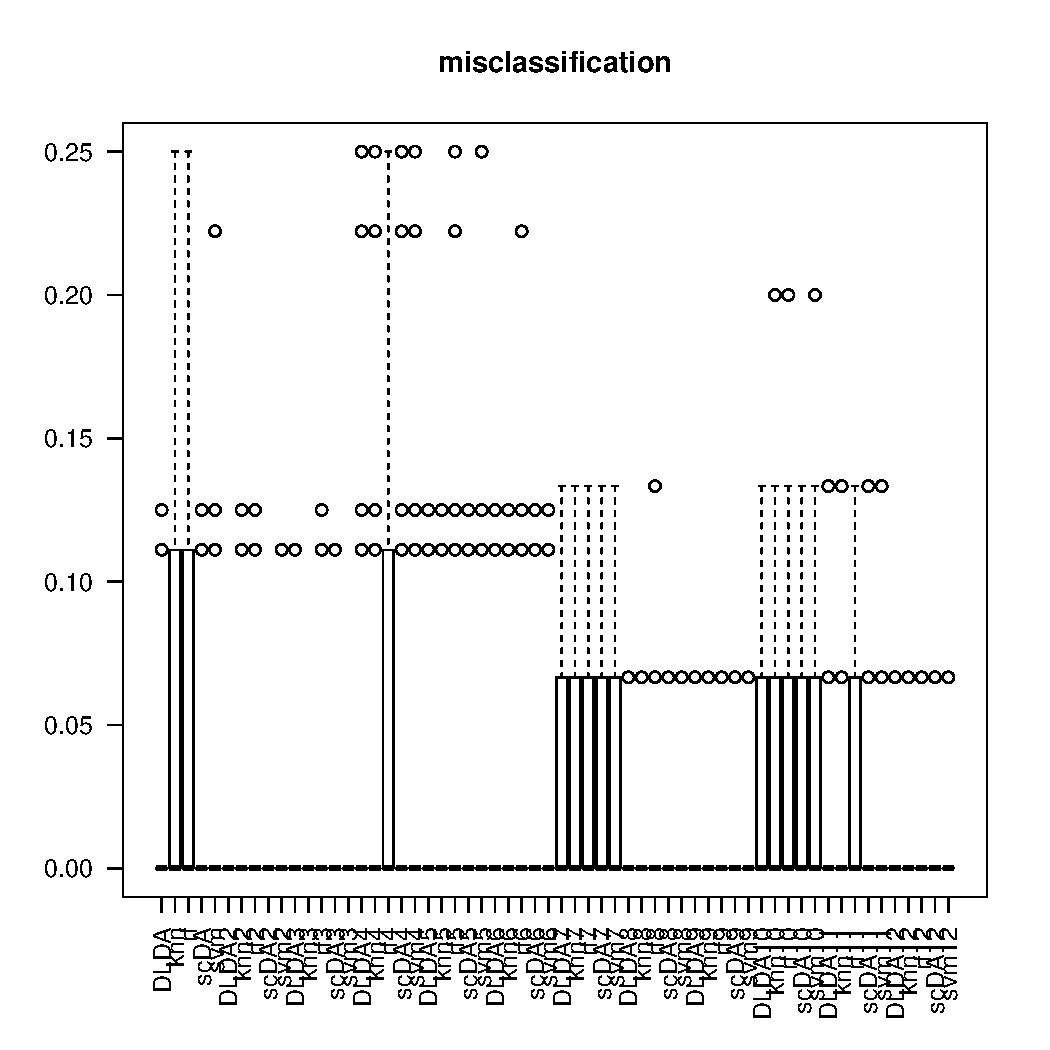
\includegraphics[width=\maxwidth]{images/graficclassify1Eval-1} 

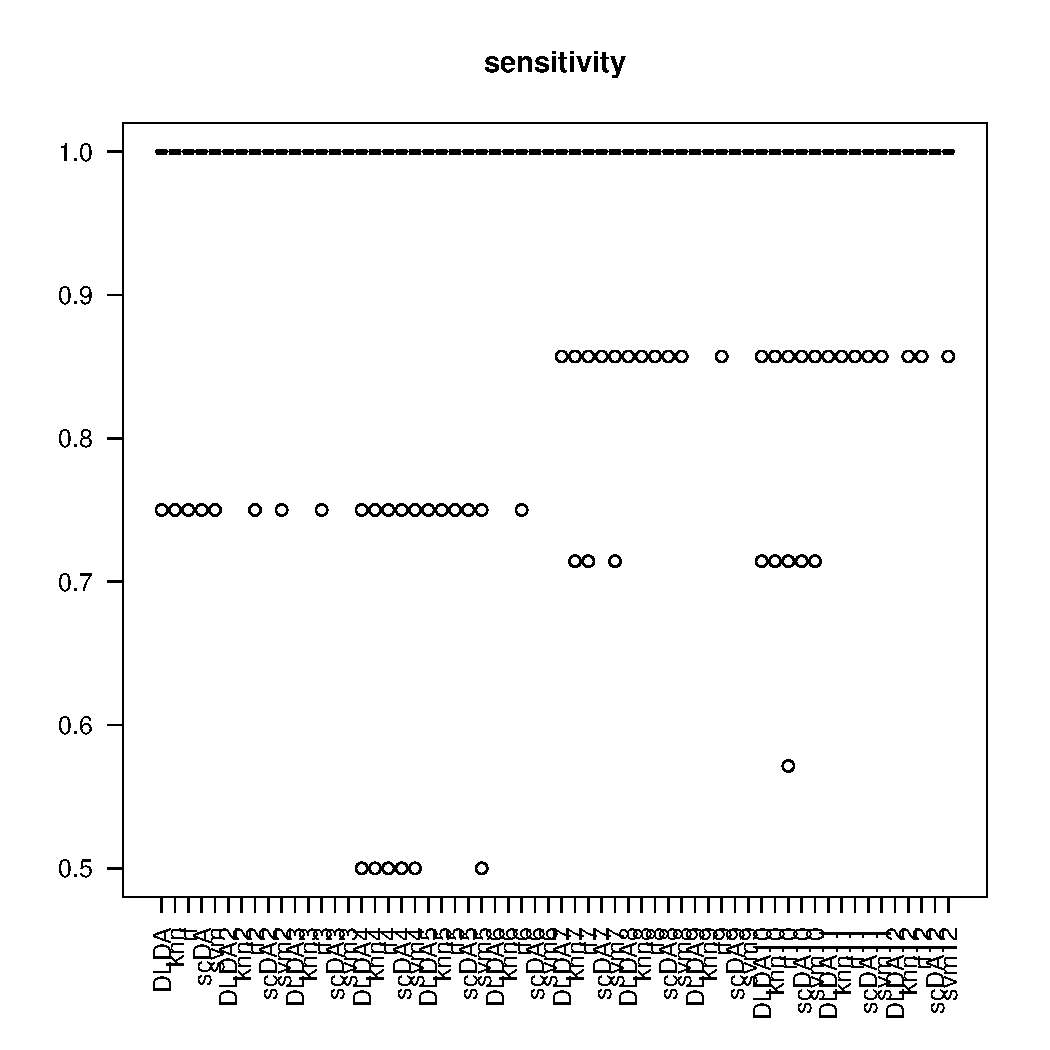
\includegraphics[width=\maxwidth]{images/graficclassify1Eval-2} 

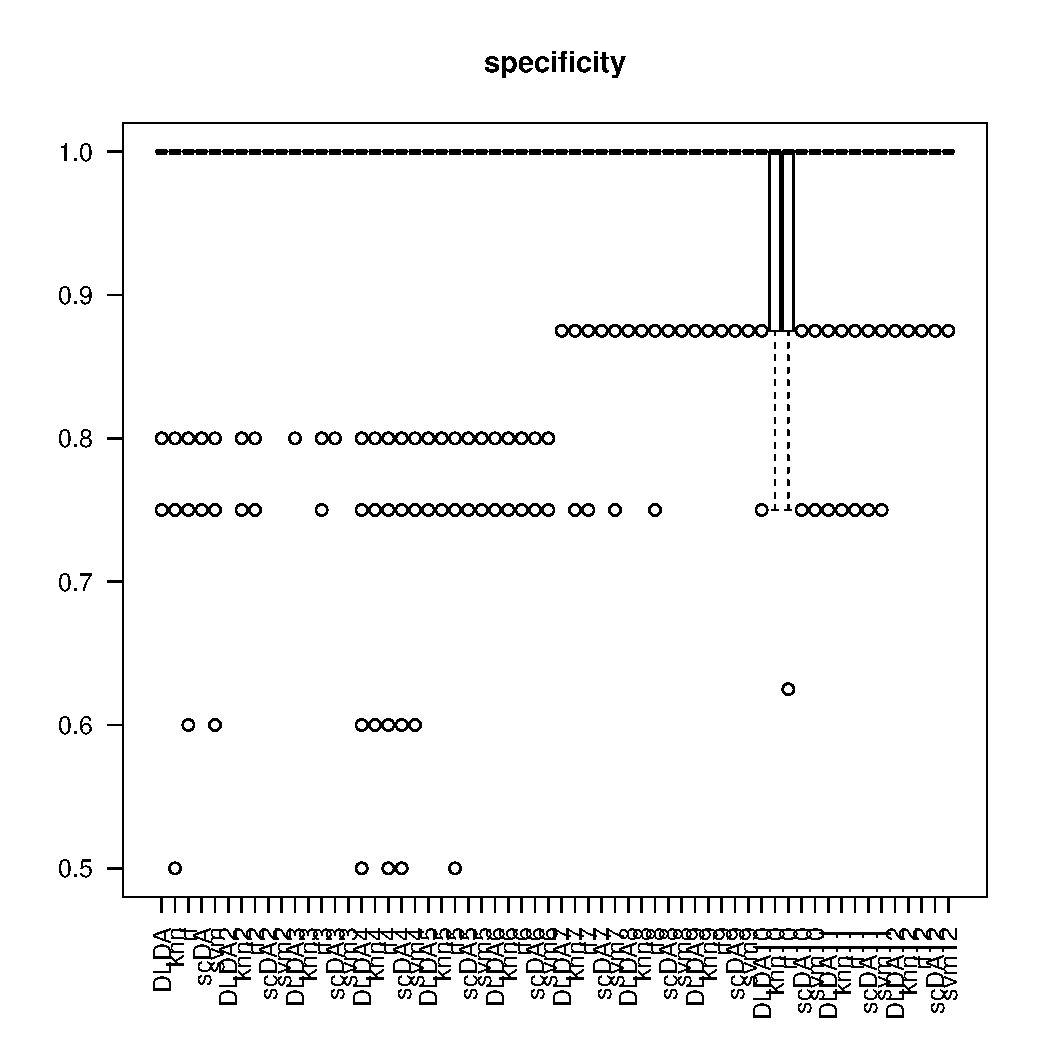
\includegraphics[width=\maxwidth]{images/graficclassify1Eval-3} 
\begin{kframe}\begin{alltt}
\hlstd{resultsClassif} \hlkwb{<-} \hlkwd{data.frame}\hlstd{(}\hlkwc{CrossVal}\hlstd{=s1,} \hlkwc{VarSel}\hlstd{=s2,}
                             \hlkwc{numGenes}\hlstd{=s3,} \hlkwc{Classif}\hlstd{=s4,compClassifs)}
\end{alltt}


{\ttfamily\noindent\color{warningcolor}{\#\# Warning in data.frame(CrossVal = s1, VarSel = s2, numGenes = s3, Classif = s4, : row names were found from a short variable and have been discarded}}\begin{alltt}
\hlkwd{write.csv2}\hlstd{(resultsClassif,}
           \hlkwc{file}\hlstd{=}\hlkwd{file.path}\hlstd{(resultsDir,}
                          \hlkwd{paste}\hlstd{(}\hlstr{"resultsClassif"}\hlstd{,}
                                \hlstd{numIter,} \hlstr{"csv"}\hlstd{,} \hlkwc{sep}\hlstd{=}\hlstr{"."}\hlstd{)))}
\end{alltt}
\end{kframe}
\end{knitrout}

\bibliography{reviewmicroarrays} 

\end{document}
